% 1958 年江苏卷第 5 题：圆内接四边形 ABCD（AB 为水平直径，D、C 在上半圆，D 约 115°、C 约 56° 方向），连 AD、DC、CB 与对角线 AC、DB；源卷图无顶点圆点、无圆心标记，故不标（按源卷布局）
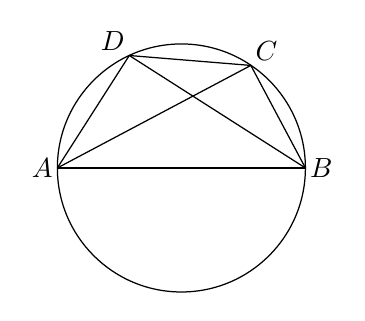
\begin{tikzpicture}[scale=1.05, line width=0.45pt,
  every node/.style={inner sep=1.5pt}]
  \coordinate (A) at (-1.5,0);
  \coordinate (B) at (1.5,0);
  \coordinate (D) at (-0.63,1.36);
  \coordinate (C) at (0.84,1.24);
  \draw (0,0) circle (1.5);
  \draw (A) -- (B);
  \draw (A) -- (D);
  \draw (D) -- (C);
  \draw (C) -- (B);
  \draw (A) -- (C);
  \draw (D) -- (B);
  \node[anchor=east] at (A) {$A$};
  \node[anchor=west] at (B) {$B$};
  \node[anchor=south east] at (D) {$D$};
  \node[anchor=south west] at (C) {$C$};
\end{tikzpicture}
